% Compile from this directory with: ../../tmp/latex-env/Library/bin/tectonic.exe progress_report.tex
% Figures are generated by the repository's EDA/experiment scripts and live in sibling report folders.
\documentclass[aspectratio=169,11pt]{beamer}
\usepackage[T1]{fontenc}
\usepackage{lmodern}
\usepackage{graphicx}
\usepackage{booktabs}
\usepackage{xcolor}

\definecolor{ink}{HTML}{193247}
\definecolor{teal}{HTML}{147D91}
\definecolor{orange}{HTML}{DF7B2D}
\definecolor{muted}{HTML}{52697C}
\setbeamercolor{normal text}{fg=ink,bg=white}
\setbeamercolor{structure}{fg=teal}
\setbeamercolor{frametitle}{fg=ink,bg=white}
\setbeamercolor{title}{fg=ink}
\setbeamercolor{block title}{fg=white,bg=teal}
\setbeamercolor{block body}{fg=ink,bg=teal!8}
\setbeamertemplate{navigation symbols}{}
\setbeamertemplate{itemize item}{\color{orange}$\bullet$}
\setbeamertemplate{footline}{\hfill\color{muted}\insertframenumber\,/\,15\hspace{0.55cm}\vspace{0.25cm}}
\setbeamerfont{frametitle}{size=\Large,series=\bfseries}
\setbeamerfont{title}{size=\huge,series=\bfseries}
\setbeamerfont{subtitle}{size=\Large}
\setbeamersize{text margin left=0.72cm,text margin right=0.72cm}
\newcommand{\src}[1]{\par\vfill{\tiny\color{muted}Source: \texttt{\detokenize{#1}}}}
\newcommand{\takeaway}[1]{\par\vspace{0.15cm}{\color{teal}\bfseries #1}}

\title{Predicting HDB monthly rent in Singapore}
\subtitle{CS5228 project progress report}
\date{October 2026}

\begin{document}

% 1
\begin{frame}[plain]
  \vspace{1.35cm}
  {\color{teal}\large CS5228 DATA MINING PROJECT}\par\vspace{0.55cm}
  {\usebeamerfont{title}\inserttitle}\par\vspace{0.42cm}
  {\usebeamerfont{subtitle}\color{muted}\insertsubtitle}\par\vspace{1.05cm}
  {\large October 2026}\par\vspace{0.18cm}
  {\color{muted}Internal out-of-time validation; no Kaggle test score reported}
\end{frame}

% 2
\begin{frame}{Task, data and evaluation question}
  \begin{columns}[T,onlytextwidth]
  \begin{column}{0.52\textwidth}
    \textbf{Target}\quad Monthly approved rent (SGD) for an individual HDB rental record.\par\vspace{0.22cm}
    \textbf{Labeled train}\quad 150,000 rows, Jan 2021--Mar 2025.\par\vspace{0.22cm}
    \textbf{Unlabeled test}\quad 50,000 rows, Mar 2025--Jul 2026; 49,620 postdate the final train month.
  \end{column}
  \begin{column}{0.45\textwidth}
    \textbf{Project questions}\par\vspace{0.12cm}
    \begin{itemize}\setlength\itemsep{0.14cm}
      \item What do property, time and location explain?
      \item Do blocks and amenities improve prediction?
      \item Do COE and stocks add a reliable leading signal?
    \end{itemize}
  \end{column}
  \end{columns}
  \takeaway{Most test rows are future-dated: validation must move forward in time.}
  \src{reports/train_test_eda/summary.json; CS5228 project brief (provided)}
\end{frame}

% 3
\begin{frame}{Data audit: clean core table, but important caveats}
  \small
  \begin{tabular}{@{}p{3.05cm}p{8.05cm}@{}}
    \toprule
    Check & Observed result and treatment \\
    \midrule
    Missing/duplicates & No empty core cells; 425 exact train duplicates. Retain ambiguous copies because there is no rental ID to prove error. \\
    Constant fields & \texttt{FURNISHED} is always yes; \texttt{FEE} is always zero. Exclude from learning. \\
    Inconsistency & One lease-commencement year exceeds approval year; flag the resulting age rather than assuming it is valid. \\
    Categories & Normalize labels such as \texttt{4 room} / \texttt{4-room}; fit categorical encoding on training months only. \\
    Auxiliary sentinels & Treat block \texttt{NIL} and \texttt{-1} as missing, not physical values. \\
    \bottomrule
  \end{tabular}
  \vspace{0.13cm}\par
  \small The stock file also has missing quote fields; its data quality is separate from the complete rental table.
  \src{reports/train_test_eda/summary.json; reports/auxiliary_data_eda/summary.json}
\end{frame}

% 4
\begin{frame}{Property EDA: rent spread, size and flat type}
  \begin{columns}[T,onlytextwidth]
  \begin{column}{0.52\textwidth}
    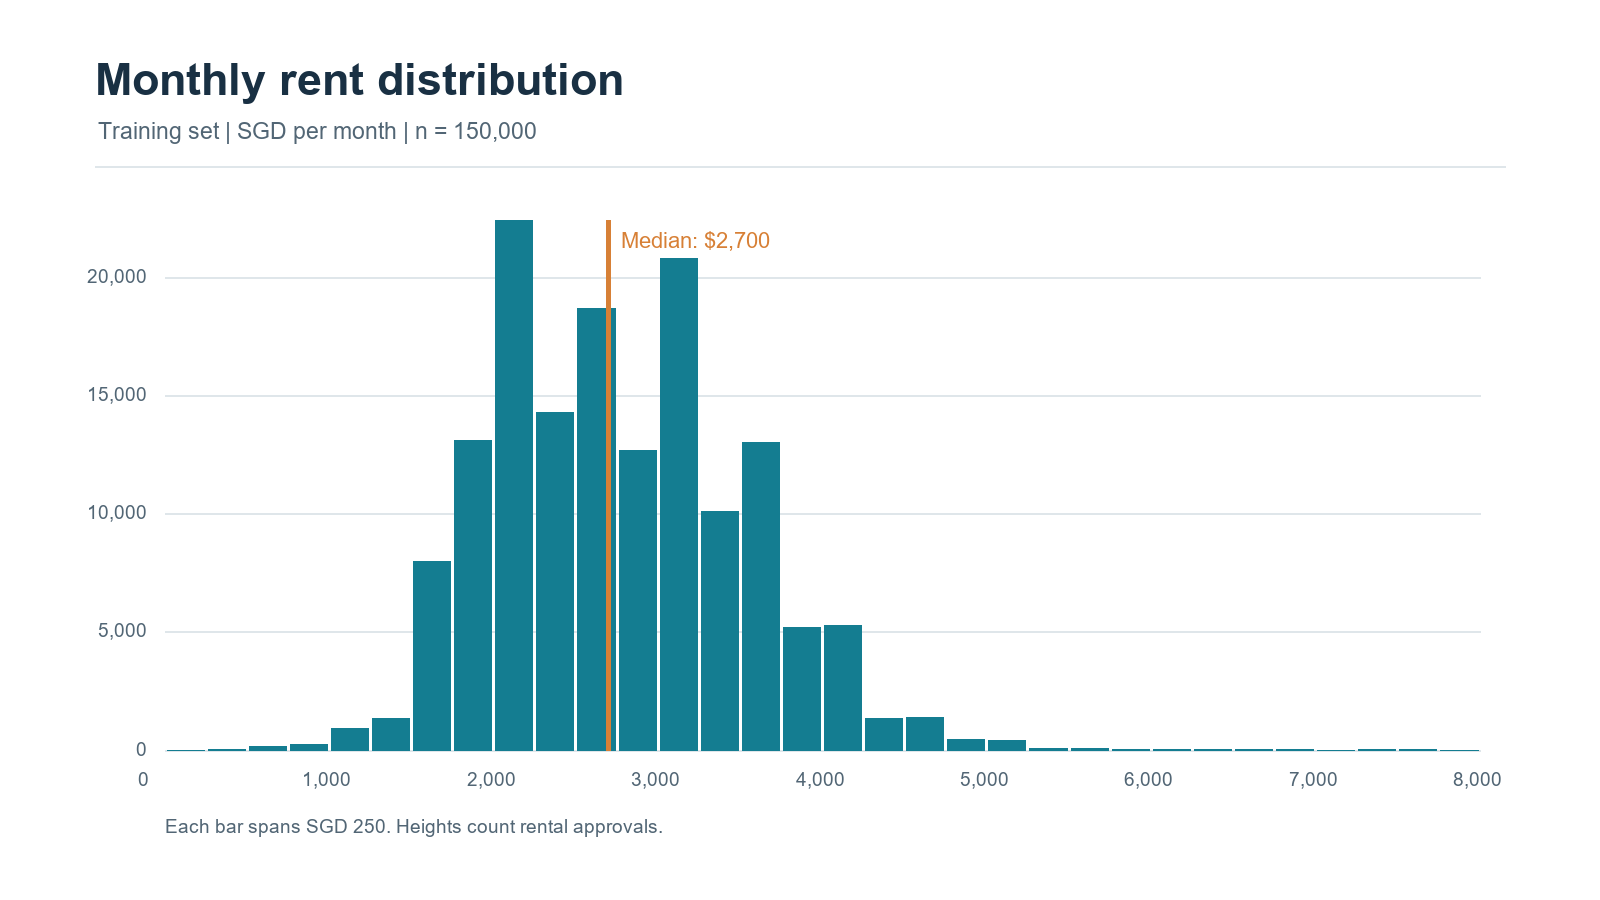
\includegraphics[width=\linewidth]{../train_test_eda/01_rent_distribution.png}
  \end{column}
  \begin{column}{0.45\textwidth}
    \small
    \begin{tabular}{@{}lrr@{}}
      \toprule
      Flat type & $n$ & Median SGD \\
      \midrule
      2-room & 3,098 & 2,100 \\
      3-room & 49,024 & 2,350 \\
      4-room & 54,079 & 2,800 \\
      5-room & 35,523 & 3,000 \\
      Executive & 8,234 & 3,000 \\
      \bottomrule
    \end{tabular}\par\vspace{0.13cm}
    Area: 31--215 m$^2$; raw area--rent $r=0.329$. One-room: just 42 rows.
  \end{column}
  \end{columns}
  \small Rent: min 300; Q1 2,100; median 2,700; Q3 3,200; P95 4,000; P99 4,600; max 7,600 SGD. Raw associations can reflect other features.
  \src{reports/train_test_eda/summary.json; reports/train_test_eda/01_rent_distribution.png}
\end{frame}

% 5
\begin{frame}{Temporal EDA: a strong nonstationary level}
  \centering
  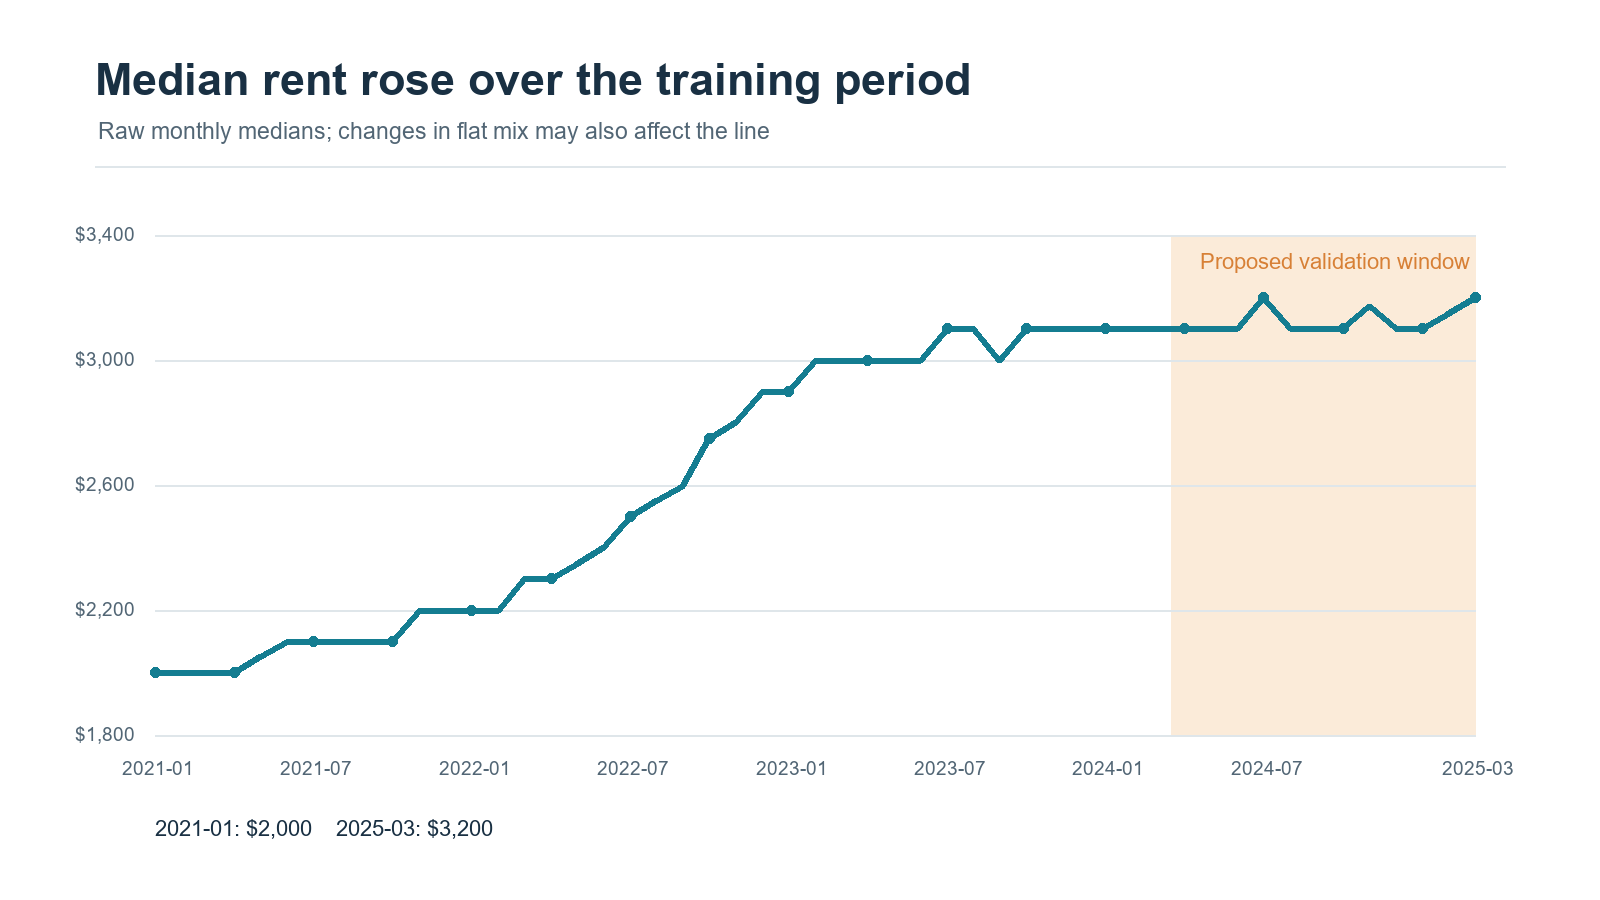
\includegraphics[width=0.61\linewidth]{../train_test_eda/02_monthly_median.png}\par
  \vspace{0.02cm}
  \small Raw monthly median rent rose from SGD 2,000 (Jan 2021) to SGD 3,200 (Mar 2025). This is a 60\% level increase, not necessarily a same-flat appreciation estimate.\par
  \takeaway{Month, recency and a forward holdout belong in the baseline.}
  \src{reports/train_test_eda/summary.json; reports/train_test_eda/02_monthly_median.png}
\end{frame}

% 6
\begin{frame}{Spatial EDA: town heterogeneity and block coverage}
  \begin{columns}[T,onlytextwidth]
  \begin{column}{0.51\textwidth}
    \small
    \begin{tabular}{@{}l@{\hspace{0.25cm}}r@{\hspace{0.25cm}}r@{}}
      \toprule
      Selected town & $n$ & Median SGD \\
      \midrule
      Bukit Timah & 438 & 3,000 \\
      Central & 2,278 & 3,000 \\
      Bishan & 3,306 & 2,900 \\
      Punggol & 6,668 & 2,850 \\
      Bedok & 8,907 & 2,500 \\
      Yishun & 7,913 & 2,500 \\
      \bottomrule
    \end{tabular}
  \end{column}
  \begin{column}{0.46\textwidth}
    \small
    Across 26 towns, median rent ranges from SGD 2,500 to 3,000. Town sizes and flat mixes differ.\par\vspace{0.16cm}
    Normalized town--block--street keys match \textbf{100\%} of train and test rows to 9,464 block records.\par\vspace{0.16cm}
    Coordinates, planning area, subzone, completion year and maximum floor add within-town detail.
  \end{column}
  \end{columns}
  \src{reports/train_test_eda/summary.json; reports/auxiliary_data_eda/summary.json}
\end{frame}

% 7
\begin{frame}{Amenity EDA: accessible, but snapshot-based}
  \begin{columns}[T,onlytextwidth]
  \begin{column}{0.55\textwidth}
    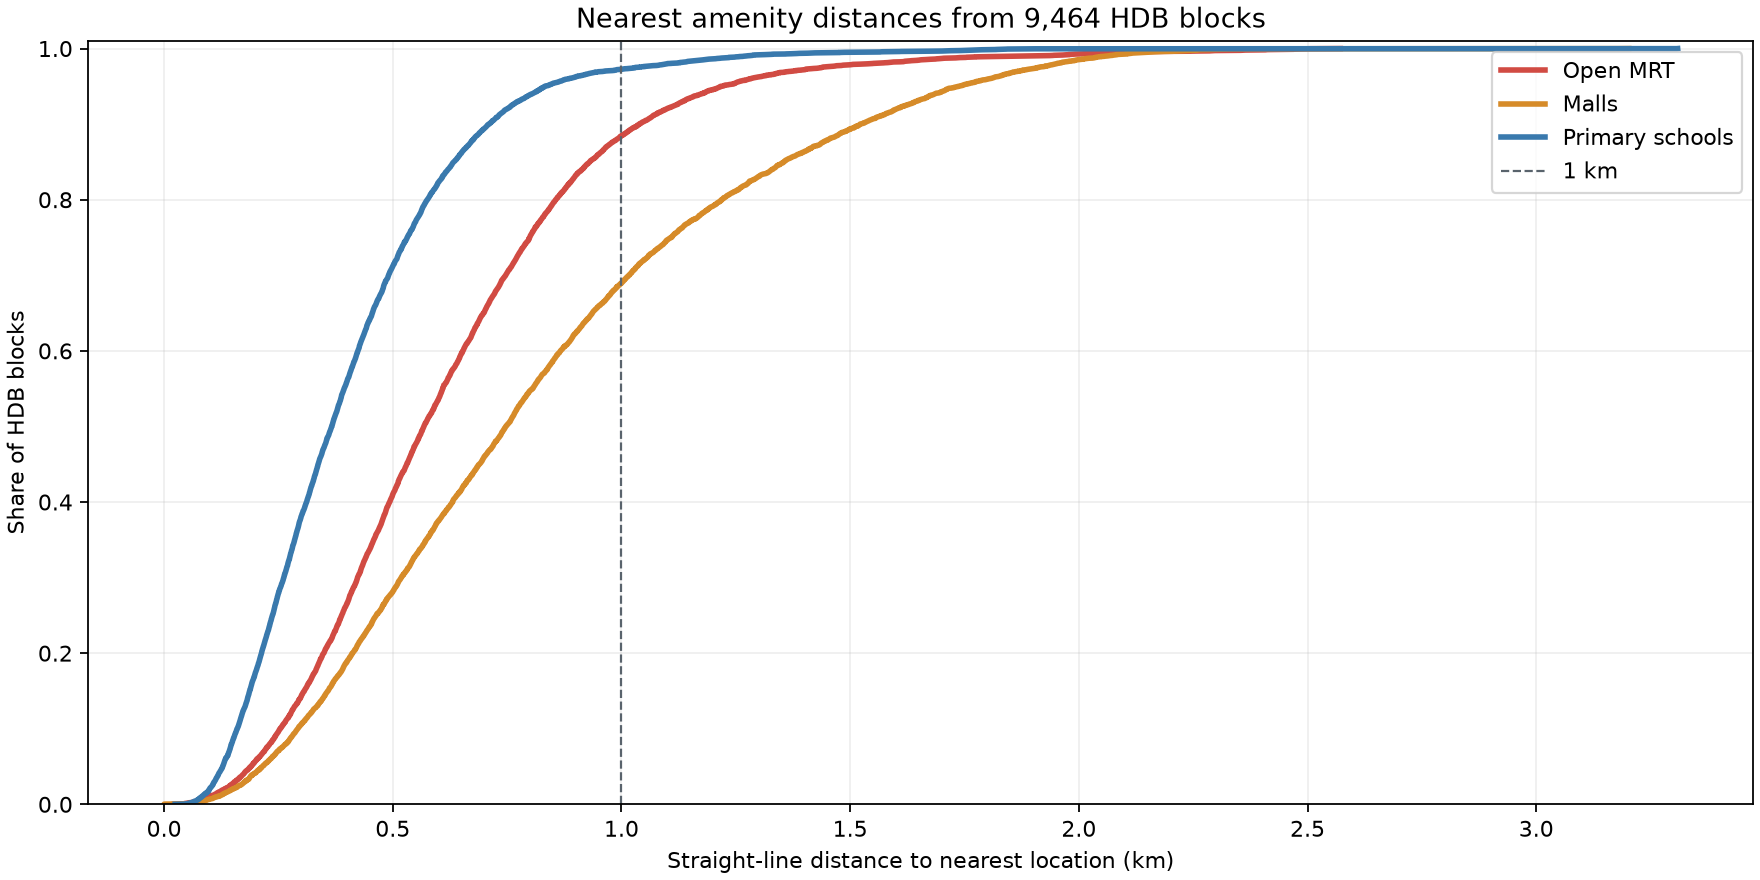
\includegraphics[width=\linewidth]{../auxiliary_data_eda/02_nearest_distances.png}
  \end{column}
  \begin{column}{0.42\textwidth}
    \small
    \begin{tabular}{@{}lrr@{}}
      \toprule
      Nearest & Median km & $\leq$1 km \\
      \midrule
      MRT & 0.568 & 88.46\% \\
      Mall & 0.747 & 68.97\% \\
      Primary school & 0.366 & 97.23\% \\
      \bottomrule
    \end{tabular}\par\vspace{0.16cm}
    192 unique open MRT locations, 113 malls and 180 unique primary-school locations feed straight-line distance and count features.
  \end{column}
  \end{columns}
  \small Facility files are current snapshots: historical opening/closure dates are not available, so temporal interpretation is limited.
  \src{reports/auxiliary_data_eda/summary.json; reports/auxiliary_data_eda/02_nearest_distances.png}
\end{frame}

% 8
\begin{frame}{Economic associations have not yielded stable row-level gains}
  \small
  \begin{tabular}{@{}llr@{}}
    \toprule
    Pair of monthly series & Transformation & Pearson $r$ \\
    \midrule
    Raw mean rent vs COE C premium & Levels; COE lag 1 & +0.960 \\
    Mix-adjusted rent vs COE C & Growth; COE lag 1 & +0.306 \\
    Mix-adjusted rent vs SG stock & Growth/return; lag 1 & $-0.181$ \\
    \bottomrule
  \end{tabular}\par\vspace{0.18cm}
  \small Growth correlations use about 37 prevalidation months. The mix-adjusted rent index controls flat type/model, town, area and lease start; its adjustment is fitted before Apr 2024.\par\vspace{0.13cm}
  \small Against the same E baseline, adding engineered COE and SG-stock features together worsened row-level RMSE in all four forward windows by SGD 0.31--3.84. Individual economic sets sometimes helped a window slightly, but not consistently.\par\vspace{0.08cm}
  \takeaway{Monthly association is not evidence of a stable forward prediction gain.}
  \src{reports/temporal_correlations/pair_correlations.csv; reports/economic_feature_ablation/forward_scores.csv}
\end{frame}

% 9
\begin{frame}{Grouped time series: descriptive signal, mixed forecasts}
  \small
  \begin{columns}[T,onlytextwidth]
  \begin{column}{0.48\textwidth}
    \textbf{Planning-area correlations}\par\vspace{0.10cm}
    Lagged COE C bids-to-quota ratio vs area rent growth, across 24 eligible areas:\par\vspace{0.09cm}
    \begin{tabular}{@{}lrr@{}}
      \toprule
      Rent statistic & Positive & Median $r$ \\
      \midrule
      Mean & 20/24 & +0.148 \\
      Median & 17/24 & +0.089 \\
      \bottomrule
    \end{tabular}\par\vspace{0.13cm}
    Correlation is modest; neither sign nor magnitude establishes a causal effect.
  \end{column}
  \begin{column}{0.49\textwidth}
    \textbf{Pooled panel Ridge, median-rent RMSE}\par\vspace{0.10cm}
    \begin{tabular}{@{}lrr@{}}
      \toprule
      Forward start & +COE & +stocks \\
      \midrule
      Jan 2023 & +22.63 & +16.78 \\
      Jul 2023 & +9.78 & +1.24 \\
      Apr 2024 & $-17.50$ & $-2.76$ \\
      \bottomrule
    \end{tabular}\par\vspace{0.10cm}
    Deltas are SGD vs history-only; positive is worse. This one-step setup uses the \emph{observed} prior-month rent, unlike batch test forecasting.
  \end{column}
  \end{columns}
  \src{reports/group_temporal_panel/report.md; reports/group_temporal_panel/group_correlations.csv}
\end{frame}

% 10
\begin{frame}{Baseline protocol and leakage controls}
  \small
  \begin{itemize}\setlength\itemsep{0.13cm}
    \item \textbf{Forward split:} fit Jan 2021--Mar 2024 (114,842 rows); hold out Apr 2024--Mar 2025 (35,158 rows).
    \item \textbf{Target and metrics:} record-level rent in SGD; compare RMSE, MAE, mean prediction bias, and month-level errors.
    \item \textbf{Seven core features:} flat type, model, area, age, approval month index, month-of-year, town.
    \item \textbf{Preprocessing:} normalize labels; learn imputation, scaling and categorical encoding from fit months only.
    \item \textbf{Ablation:} add block, amenity, COE and stock groups on identical rows, split and model settings.
    \item \textbf{Forecasting caveat:} one-month-updated signals differ from a fixed-origin forecast for all future test months.
  \end{itemize}
  \src{reports/model_baseline/results.json; reports/model_families/results.json; reports/auxiliary_ablation/results.json}
\end{frame}

% 11
\begin{frame}{Baselines: feature groups change the answer}
  \small
  \begin{tabular}{@{}p{5.0cm}rrr@{}}
    \toprule
    Model / cumulative feature group & RMSE & MAE & Bias \\
    \midrule
    Fit-period mean, no features & 846.75 & 690.60 & $-531.44$ \\
    CatBoost A: type, model, area & 761.42 & 647.22 & $-534.06$ \\
    CatBoost B: A + time/age & 529.96 & 397.86 & $-49.91$ \\
    CatBoost C: B + town & \textbf{487.22} & \textbf{364.09} & $-48.29$ \\
    \bottomrule
  \end{tabular}\par\vspace{0.22cm}
  \small All scores are Apr 2024--Mar 2025 row-level SGD errors. CatBoost: 400 iterations, depth 6, learning rate 0.05, $L_2=3$, seed 42. No tuning on the test file.\par\vspace{0.10cm}
  \takeaway{Time and age are added together in B; the A-to-B gain is not time's isolated contribution.}
  \src{reports/model_baseline/model_metrics.csv; reports/model_baseline/results.json}
\end{frame}

% 12
\begin{frame}{Model-family check on the same seven core features}
  \small
  \begin{tabular}{@{}lrrr@{}}
    \toprule
    Model & RMSE & MAE & Bias \\
    \midrule
    Ridge regression ($\alpha=10$) & 624.88 & 468.18 & +361.99 \\
    Random forest (160 trees, depth 18) & 493.77 & 370.19 & $-56.65$ \\
    CatBoost (400 trees, depth 6) & 487.22 & 364.09 & $-48.29$ \\
    \color{teal}\bfseries LightGBM (400 trees, 31 leaves) & \color{teal}\bfseries 485.09 & 361.41 & $-42.68$ \\
    \bottomrule
  \end{tabular}\par\vspace{0.22cm}
  \small Same 35,158-row holdout and seven features, with model-appropriate preprocessing. Ridge has a strong positive mean bias; trees handle nonlinear property/location effects better here.\par\vspace{0.12cm}
  \takeaway{LightGBM leads CatBoost by only SGD 2.12 RMSE on this single split.}
  \src{reports/model_families/family_metrics.csv; reports/model_families/results.json}
\end{frame}

% 13
\begin{frame}{Auxiliary ablation: blocks and amenities help most}
  \small
  \begin{tabular}{@{}l@{\hspace{0.22cm}}r@{\hspace{0.22cm}}r@{\hspace{0.22cm}}r@{}}
    \toprule
    HistGradientBoosting feature set & Features & RMSE & Bias \\
    \midrule
    A: property & 3 & 758.51 & $-531.85$ \\
    B: + time/age & 6 & 527.21 & $-48.35$ \\
    C: + town & 7 & 485.72 & $-46.78$ \\
    D: + block attributes & 15 & 480.22 & $-46.90$ \\
    \textcolor{teal}{\textbf{E: + amenities}} & 29 & \textcolor{teal}{\textbf{478.82}} & $-46.16$ \\
    F: + COE & 41 & 480.66 & $-62.72$ \\
    G: + stocks & 47 & 481.31 & $-65.93$ \\
    H: + interactions & 50 & 481.58 & $-71.83$ \\
    \bottomrule
  \end{tabular}\par\vspace{0.10cm}
  \small Same model (200 boosting iterations, 31 leaves, learning rate 0.05) and holdout throughout. E improves over C by SGD 6.89 RMSE (1.42\%). F/G test the original macro feature sets; both worsen this split. A separate engineered-signal comparison also finds no consistent forward gain. Do not compare this ablation to LightGBM as a pure feature effect.
  \src{reports/auxiliary_ablation/ablation_metrics.csv; reports/economic_feature_ablation/forward_scores.csv}
\end{frame}

% 14
\begin{frame}{Diagnostics: useful signals, persistent drift}
  \small
  \begin{columns}[T,onlytextwidth]
  \begin{column}{0.51\textwidth}
    \textbf{E: block + amenities}\par\vspace{0.10cm}
    RMSE 478.82; MAE 356.36; mean bias $-46.16$ SGD. In Mar 2025, RMSE 457.45 but bias $-80.10$: average underprediction persists.\par\vspace{0.16cm}
    CatBoost C has RMSE 594.62 on 1,778 executive-flat holdout rows; only 14 one-room rows are too sparse for a stable slice.
  \end{column}
  \begin{column}{0.46\textwidth}
    \textbf{E permutation importance}\par\vspace{0.10cm}
    Largest MSE increases in a 2,000-row validation sample: flat type 151k, subzone 100k, area 31.6k; nearest mall 2.5k and MRT 2.3k.\par\vspace{0.16cm}
    Correlated features can share importance; this is predictive reliance, not an amenity price effect.
  \end{column}
  \end{columns}
  \takeaway{More forward splits and month-/group-level error audits matter more than a tiny single-split gain.}
  \src{reports/auxiliary_ablation/feature_importance.csv; reports/auxiliary_ablation/monthly_errors.csv; reports/model_baseline/flat_type_errors.csv}
\end{frame}

% 15
\begin{frame}{Current conclusion and next experiments}
  \small
  \textbf{Current evidence}\par\vspace{0.09cm}
  Property, time/age, block and amenity features improve the current row-level baseline. Some economic indicators show monthly associations and a late grouped one-step gain, but the tested economic feature sets have not delivered a stable row-level forward improvement.\par\vspace{0.20cm}
  \textbf{Next experiments}\par\vspace{0.06cm}
  \begin{enumerate}\setlength\itemsep{0.10cm}
    \item Keep E as the feature benchmark; test leading model families on the same expanded set.
    \item Repeat fixed-origin splits at a horizon near the future test span; test recency and group trends without future observed rent.
    \item Revisit only availability-safe economic lags if they improve those tests; audit historical amenity coverage and sparse groups before final refit.
  \end{enumerate}
  \src{reports/auxiliary_ablation/results.json; reports/group_temporal_panel/report.md; reports/economic_feature_ablation/forward_scores.csv}
\end{frame}

\end{document}
